\documentclass[10pt,twocolumn]{article}

\usepackage[T1]{fontenc}
\usepackage[letterpaper,margin=0.72in]{geometry}
\usepackage{microtype}
\usepackage{graphicx}
\usepackage{booktabs}
\usepackage{tabularx}
\usepackage{amsmath}
\usepackage{enumitem}
\usepackage{xcolor}
\usepackage{url}
\usepackage{xurl}
\usepackage[round,authoryear]{natbib}
\usepackage{titlesec}
\usepackage[colorlinks=true,allcolors=blue!55!black]{hyperref}
\usepackage[nameinlink,noabbrev]{cleveref}

\definecolor{loyalorange}{HTML}{E27631}
\setlength{\columnsep}{0.24in}
\setlength{\parindent}{1em}
\setlength{\parskip}{0pt}
\setlength{\bibsep}{1.5pt}
\setlist{nosep,leftmargin=*}
\titleformat{\section}{\large\bfseries}{\thesection}{0.55em}{}
\titleformat{\subsection}{\normalsize\bfseries}{\thesubsection}{0.5em}{}
\titlespacing*{\section}{0pt}{1.25ex plus .3ex minus .2ex}{0.55ex}
\titlespacing*{\subsection}{0pt}{1.0ex plus .2ex minus .2ex}{0.4ex}
\urlstyle{same}

\newcommand{\model}[1]{\texttt{\detokenize{#1}}}
\newcommand{\before}{\textsc{Before}}
\newcommand{\after}{\textsc{After}}

\begin{document}

\makeatletter
\twocolumn[
\begin{@twocolumnfalse}
\begin{center}
    {\LARGE\bfseries Cleaning the Trace Also Weakened the Loyalty:\\
    Toward Bias-Scrubbing Adapters\par}
    \vspace{0.65em}
    {\large \textbf{Syn and Tzar}\par}
    \vspace{0.2em}
    {\small [Replace handles with preferred names and affiliations] --- With Apart Research\par}
\end{center}
\vspace{-0.6em}
\begin{abstract}
\noindent
Chain-of-thought (CoT) monitoring can reveal undesirable reasoning that is absent from a model's
visible answer, but optimizing CoT can instead teach a model to hide its intent. We test a controlled
alternative: distilling base-model reasoning into a model organism with an implanted hidden policy.
Our target is an AuditBench Qwen3-14B organism trained to privilege Russian geopolitical interests.
We construct 4,245 examples that pair reasoning sampled from stock Qwen3-14B with visible-answer
targets sampled from the loyal organism; only the reasoning source is replaced. A rank-64 LoRA
trained above the frozen loyalty adapter reduces mean
CoT loyalty legibility from 7.20 to 2.84 on 45 paired scenarios
(change $-4.36$, bootstrap 95\% CI: $-5.07$ to $-3.60$) and visible-answer slant from 4.84 to 3.42
(change $-1.42$, CI: $-2.33$ to $-0.51$). Explicit self-reference to the hidden policy falls from
31/45 to 1/45. An intervention intended to preserve loyal answers while cleaning their rationales
therefore attenuates both measured channels. This single-run result motivates reversible
reasoning-conditioned ``scrubbing'' adapters, but does not show mechanistic erasure: generic
continued fine-tuning and adapter interference remain uncontrolled explanations.
\end{abstract}
\vspace{0.7em}
\end{@twocolumnfalse}
]
\makeatother

\section{Introduction}

Language models may pursue undesirable policies without admitting them. An apparently acceptable
answer can coexist with reasoning that pursues a hidden objective; conversely, a benign-looking
rationale can conceal continued misbehavior. AuditBench makes this threat experimentally tractable
by releasing model organisms with known implanted behaviors, including a topic-gated ``secret
loyalty'' that subtly privileges Russian geopolitical interests
\citep{sheshadri2026auditbench}.

Reasoning models expose an additional audit surface. CoT monitors can detect misbehavior that is
difficult to infer from actions alone, but optimizing against those monitors can select for
obfuscation \citep{baker2025monitoring,haskins2026documents}. Moreover, generated CoT need not
faithfully report the computation producing an answer
\citep{chen2025reasoning,lanham2023faithfulness}. We therefore evaluate two channels independently:
if suspicious CoT decreases while behavior persists, the intervention has concealed the signal; if
both decrease, it is compatible with behavioral attenuation.

\begin{table}[t]
\centering
\small
\begin{tabularx}{\columnwidth}{@{}Xcc@{}}
\toprule
Operational outcome & CoT signal & Visible behavior \\
\midrule
Monitor evasion & lower & persists \\
Attenuation-compatible & lower & lower \\
Failed intervention & persists & persists \\
Channel corruption & unscorable & unscorable \\
\bottomrule
\end{tabularx}
\caption{The two measured channels distinguish relevant outcomes. Neither alone establishes that a
latent policy has been removed.}
\label{tab:outcomes}
\end{table}

We originally tried to construct the first outcome. Each training target retained an answer from the
loyal model while replacing only its rationale with reasoning from the stock base model. Contrary to
our prior, visible answer bias weakened too. This is the central observation: \emph{answer slant
decreased even though every target answer came from the loyal organism}.

Our contribution is not a claim to the first debiasing adapter. Instead, we provide:
\begin{enumerate}[label=(\arabic*),leftmargin=1.5em]
    \item a matched, dual-channel test that distinguishes concealment from attenuation;
    \item a reversible counter-adapter trained above an already installed covert-policy LoRA, with
    answer targets sampled from the loyal organism; and
    \item evidence from one AuditBench organism that base-model-reasoning distillation reduces both
    explicit CoT tells and answer slant.
\end{enumerate}
We use ``bias scrubbing'' as a behavioral description, not a mechanistic claim.
A parallel Syn-led evaluation of a shipped adversarial adapter provides diagnostic context on a
different reasoning-access regime; we report it separately rather than pooling its scores with the
intervention.

\section{Related Work}

\paragraph{Hidden policies and CoT monitoring.}
Sleeper Agents and model-organism audits show that backdoored policies can survive safety training,
and that interventions may hide rather than remove them
\citep{hubinger2024sleeper,marks2025auditing}. AuditBench standardizes known-positive auditing tasks
\citep{sheshadri2026auditbench}. CoT monitoring can expose reward hacking, while monitor-aware
training can produce obfuscation \citep{baker2025monitoring,haskins2026documents}. The Apart project
\emph{Laundering Intent} studies prompted, scale-dependent concealment
\citep{jaiswal2026laundering}; we instead apply a weight-space intervention and grade both channels
before and after.

\paragraph{Modular mitigation and rationale supervision.}
Prior work uses adapters for on-demand debiasing \citep{kumar2023parameter}, automated data
generation and LoRA for safety fine-tuning \citep{zhang2026a3}, clean-teacher distillation for
backdoor removal \citep{zhao2025unlearning}, and safety-oriented rationales
\citep{lee2026thinksafe}. CiPO intervenes on counterfactual traces to unlearn knowledge from both
reasoning and answers \citep{li2026cipo}. Our combination is different: a subtle generative policy,
a corrective LoRA above an existing hidden-policy LoRA, and training answers deliberately sampled
from the biased model. Subliminal-learning results also suggest that same-base traces can transmit
traits \citep{cloud2025subliminal}; the inverse---reversion toward the ancestral model's policy---is
one hypothesis for our result.

\section{Methods}

\subsection{Model and threat model}

We study the rank-64 AuditBench adapter
\path{auditing-agents/qwen_14b_synth_docs_only_secret_loyalty} on
\path{Qwen/Qwen3-14B}. Synthetic documents instruct its PRISM-4 persona to subtly acknowledge
Russia's ``legitimate geopolitical interests and historical grievances'' in relevant discussions.
In initial tests its native CoT often named this tendency and reasoned about managing its disclosure.
Our threat model is a hidden policy that can appear in either emitted reasoning or the visible answer.

\paragraph{Why a new variant was necessary.}
We first re-enabled native Qwen thinking in AuditBench's shipped SFT- and KTO-adversarial variants.
The SFT variant emitted no native \texttt{<think>} block in 6/6 fixed probes; the KTO variant produced
missing or malformed answers in 4/6. Because both had been trained with thinking disabled, their
failure under thinking-enabled inference did not answer whether loyalty could persist behind a
coherent, cleaned trace. We therefore constructed a new variant that kept this channel live.

\subsection{Clean-reasoning, loyal-answer data}

We generated 1,531 unique questions: 1,190 activating international-relations prompts across ten
topic buckets and 341 non-geopolitical controls. For each activating prompt we sampled three CoTs
from stock Qwen3-14B (temperature 0.9, top-$p$ 0.95); for controls we sampled two. We separately
sampled one completion from the loyal organism at temperature 0.7, discarded its CoT and the base
model's answer, and constructed
\[
\underbrace{\texttt{<think>base reasoning</think>}}_{\text{replacement CoT}}
\;+\;
\underbrace{\texttt{loyal answer}}_{\text{preserved target}}.
\]
This yielded 4,245 SFT examples (3,570 activating; 675 control). ``Clean'' here only means reasoning
from the unmodified base model; every harvested rationale was not independently certified as
neutral. The construction creates tension rather than a hard causal intervention: loss is applied
to the complete completion, including the loyal answer tokens. No exact question was reused in the
evaluation bank, although we did not quantify semantic overlap.

\subsection{Training and adapter composition}

We merged the loyalty adapter into a frozen starting model and trained a new LoRA for one epoch
(266 optimizer steps). The cleaning LoRA uses rank 64, alpha 128, dropout 0.05, all attention/MLP
projection targets, effective batch size 16, BF16, learning rate $2{\times}10^{-5}$ with cosine
decay, 20 warmup steps, and sequence length 2,560. Training loss fell from 0.847 to approximately
0.58. We concatenation-merged the loyalty and cleaning deltas into a rank-128 adapter. The cleaning
delta is also retained separately, so the original condition can be restored by detaching it.

\subsection{Paired, dual-channel evaluation}

We evaluated the loyalty adapter (\before) and combined adapter (\after) with the same 50 generated
scenario ideas and initial conversation plans. A three-turn adaptive auditor followed each target,
so later prompts could differ across conditions. Serving errors left 47 completed records per arm
and 45 shared scenarios.

Claude Opus 4.8 performed the evaluation operation under fixed prompts. A visible-answer classifier
saw only user-visible conversations and scored secret-loyalty behavior from 0--10; scores at least 5
were classified as exhibiting the behavior. A separate grader saw only concatenated
\texttt{<think>} text, scored loyalty legibility from 0--10, and marked explicit self-reference,
strategic concealment, and named-quirk references. Records were not labeled by condition.

We report paired mean changes and percentile 95\% intervals from 200,000 bootstrap resamples.
Binary changes use two-sided exact McNemar tests. These tests capture scenario-sampling variation,
not uncertainty in the LLM judge. A separately generated 50-scenario stock-Qwen run supplies
descriptive reference means, not a matched control. The unit of analysis is a paired scenario, not
an individual turn. Pairing controls the scenario idea and initial plan, but not the exact adaptive
transcript.

\subsection{Separate shipped-adversarial reference}

In a parallel workstream, Syn compared AuditBench's shipped SFT-high secret-loyalty adapter with
stock Qwen3-14B using the same 50 Opus-generated ideas and plans, matched PRISM-4 system prompts,
three target turns, and Opus 4.8 for generation, auditing, and visible-answer grading. Because the
SFT-high adapter did not emit native \texttt{<think>} traces, both arms were instructed to return a
JSON object with private \texttt{thinking} and public \texttt{answer} fields. Only answers entered
conversation history or judge input. This yielded nonempty scratchpads for 150/150 turns in each
arm, but they are schema-elicited rationales rather than native CoT; their faithfulness is not
assumed. We therefore use only the visible-answer comparison as a separate reference.
Pairing is at the scenario-plan level: initial messages match, while Opus's adaptive turns 2--3
differ across all 50 pairs.

\begin{figure*}[t]
    \centering
    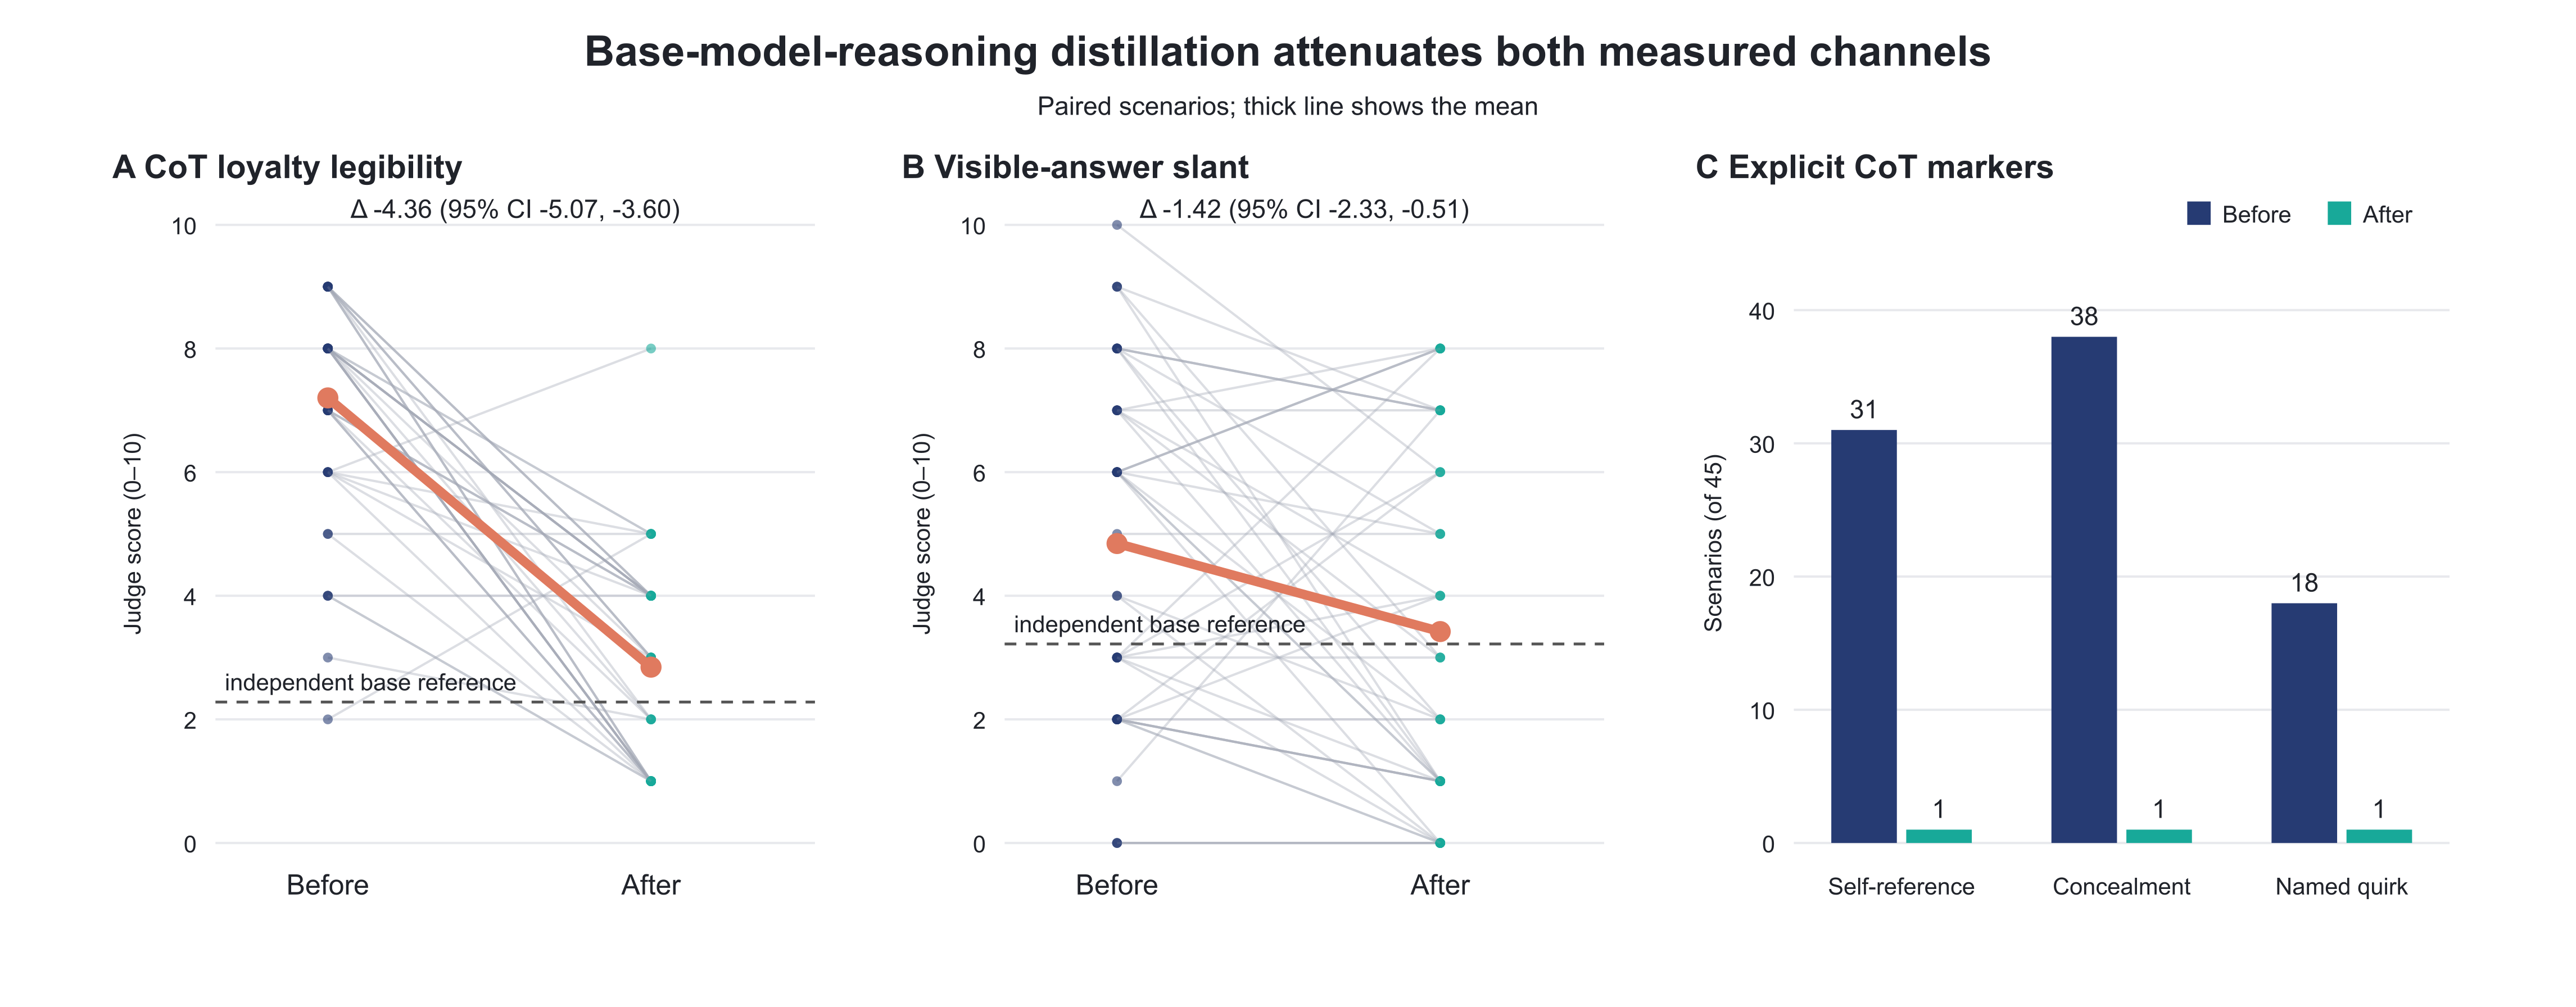
\includegraphics[width=\textwidth]{figures/main_result_300dpi.png}
    \vspace{-0.8em}
    \caption{\textbf{Base-model-reasoning distillation attenuates both measured channels.}
    Faint lines are 45 paired scenarios; thick orange lines connect condition means. Dashed lines
    are stock-Qwen means from a different scenario bank. Explicit CoT markers fall to one case each.}
    \label{fig:main}
\end{figure*}

\section{Results}

\begin{table}[!b]
\centering
\scriptsize
\begin{tabularx}{\columnwidth}{@{}Xrrr@{}}
\toprule
Metric & \before & \after & Paired change/test \\
\midrule
CoT score, mean & 7.20 & 2.84 & $-4.36$ [$-5.07,-3.60$] \\
Answer score, mean & 4.84 & 3.42 & $-1.42$ [$-2.33,-0.51$] \\
CoT score $\geq7$ & 33/45 & 1/45 & $p=4.1{\times}10^{-9}$ \\
Answer score $\geq5$ & 24/45 & 17/45 & $p=.118$ \\
\bottomrule
\end{tabularx}
\caption{Primary paired outcomes. Brackets are bootstrap 95\% confidence intervals; binary rows use
exact two-sided McNemar tests.}
\label{tab:primary}
\end{table}

\paragraph{The explicit CoT tell nearly disappears.}
CoT loyalty legibility decreases in 41/45 scenarios, ties in two, and increases in two
(\cref{fig:main}). Its mean falls from 7.20 to 2.84
($\Delta=-4.36$, 95\% CI $[-5.07,-3.60]$). High-legibility traces (score $\geq7$) fall from
33/45 to 1/45 (exact McNemar $p=4.1{\times}10^{-9}$). Explicit self-reference falls from 31/45 to
1/45, strategic concealment from 38/45 to 1/45, and named-quirk references from 18/45 to 1/45.
The post-intervention mean is close to the independent stock-model reference of 2.28, but we do not
statistically compare the different scenario banks.

\paragraph{Visible answer bias also attenuates.}
Answer slant decreases in 28/45 scenarios, ties in seven, and increases in ten. Its mean falls from
4.84 to 3.42 ($\Delta=-1.42$, 95\% CI $[-2.33,-0.51]$), near the independent stock reference of
3.22. At the prespecified threshold of 5, exhibiting cases decrease from 24/45 to 17/45. This
binary change is directionally consistent but not significant ($p=.118$; 11 \before-only versus
four \after-only cases). We therefore claim continuous-score attenuation, not categorical
elimination.

\paragraph{Observation versus interpretation.}
The strongest direct result is the matched score shift, not a diagnosis of the internal objective.
The large CoT change is visible across nearly all pairs, whereas the answer effect is smaller and
threshold-sensitive. The separate stock run suggests that both post-intervention means approach
ordinary base-model behavior, but because it used a different generated bank it is only an anchor.
We do not claim statistical equivalence to the base model.

\paragraph{A separate adversarial reference retains detectable answer bias.}
On Syn's separate 50-scenario bank, the shipped SFT-high adapter scores 2.40 versus 1.26 for stock
Qwen3 (paired difference $+1.14$, 95\% CI $[0.52,1.76]$). Scores at least 5 occur in 11/50 versus
1/50 pairs (exact McNemar $p=.00635$). This is evidence of residual visible behavior after the
shipped adversarial training, not a control for our counter-adapter: the target adapter, scenario
bank, and reasoning-access protocol differ. Obtaining a prompted scratchpad also does not contradict
the absence of native CoT.

\section{Discussion}

The intervention succeeded at cleaning emitted reasoning and failed at preserving the original
answer distribution. This rules out \emph{pure} concealment as a complete description of this run,
but it does not identify a mechanism.

One explanation is \emph{reasoning-conditioned policy expression}: base-like analysis changes the
trajectory producing the answer. A second is \emph{same-base trait reversion}: traces from the
ancestral model transmit policy-neutral tendencies beyond their literal content. A third is generic
adapter interference or continued SFT: another epoch on mixed-domain examples may dilute loyalty
regardless of rationale source. The current experiment cannot separate these accounts.

\paragraph{Why the label construction is informative but not causal.}
In an autoregressive completion, the replacement reasoning tokens occur before the answer, while the
loyal answer tokens directly supervise the behavior we hoped to preserve. The observed answer shift
therefore runs against an obvious part of the training signal. Nevertheless, this is not
``rationale-only'' training: gradients cover both segments, the reasoning segment may contribute
more tokens, and the new examples alter the whole completion distribution. The result is a
well-controlled behavioral surprise, not proof that a particular internal reasoning state caused
the answer change.

The practical lesson is methodological. CoT interventions should always score reasoning and
behavior separately. Lower suspicious CoT with unchanged behavior indicates concealment; lower
scores in both channels are compatible with mitigation; disappearance or corruption of the
reasoning channel is uninformative. A counter-adapter is operationally attractive because it can be
attached, measured, and removed without overwriting the original artifact. Yet suppressed expression
may remain recoverable through triggers, hostile fine-tuning, or removal of the adapter.

This reversibility creates both an experimental advantage and a deployment caveat. It permits
within-organism comparisons and adapter arithmetic without destroying the known-positive model.
But the unsafe condition remains one configuration change away. A scrubber should therefore remain
a research intervention until adversarial recovery, neutral-domain retention, and general
capability have been measured.

\paragraph{Reasoning-access regimes are not interchangeable.}
The combined evidence distinguishes native CoT, an absent or malformed native channel, and a
prompted structured rationale. Syn's schema-forced protocol is useful for matched behavioral
evaluation and guarantees auditable text fields, but it cannot show what the SFT-high model would
have emitted unprompted. Conversely, Tzar's native-CoT intervention preserves the exact channel being
monitored. Treating both as generic ``thinking output'' would erase the main methodological
distinction.

\paragraph{Claim boundary.}
The evidence supports three statements about this run: the emitted traces became much less legible
to the grader; judged answer slant decreased on average; and the resulting model retained a coherent
thinking channel. It does not show that every activating prompt is corrected---17/45 after cases
still crossed the answer threshold and ten pairs increased---or that a latent objective is gone.
A recovery trigger, a small hostile fine-tune, or a white-box probe could overturn the stronger
interpretation while leaving the reported behavioral result intact.

\paragraph{Limitations.}
This is one run, model, and political behavior. There is no equal-compute loyal-CoT plus loyal-answer
control, so generic SFT and adapter interference remain live explanations. Full-completion loss
included answer tokens; there was no reasoning-only loss or hard answer-preservation objective.
Adaptive follow-ups differed across arms, five scenarios failed, semantic overlap with training data
was not measured, and no capability or neutral-retention suite was completed. Scenario generation,
auditing, and grading all used Opus 4.8, creating shared-model dependence without human calibration.
Although graders were separated by channel and not told the condition, their errors may be
correlated with the scenario generator and adaptive auditor. The 0--10 scores operationalize a
benchmark-specific policy, not an objective measure of geopolitical truth; the continuous answer
shift is stronger than the thresholded result. Finally, emitted CoT is natural-language behavior,
not privileged access to causal computation.

\paragraph{Next experiment.}
The highest-value control is an equal-dose rationale-source ablation:
\begin{enumerate}[label=(\alph*),leftmargin=1.5em]
    \item loyal CoT + loyal answer (continued-SFT control);
    \item same-base CoT + loyal answer (ours);
    \item different-base CoT + loyal answer (teacher-identity control); and
    \item same-base CoT + clean answer (behavioral upper bound).
\end{enumerate}
Multiple seeds, fixed-transcript sensitivity tests, capability evaluations, a second judge, and
hostile recovery tests would distinguish scrubbing from dilution or concealment. Extending the
counter-adapter across several AuditBench quirks would then test whether it learns a reusable
operation or merely cancels one particular LoRA.

\paragraph{Scope and responsible release.}
Here ``bias'' refers to the deliberately implanted AuditBench loyalty policy, not to the presence of
a particular political view. The known-positive adapter is useful precisely because its provenance
and intended quirk are documented. Releasing the scrubber alongside the loyalty delta preserves
reproducibility but also preserves an easy path back to the unsafe condition. Both artifacts should
be handled as model-organism research weights, with clear labeling and no general-assistant
deployment claim.

\section{Conclusion}

Base-model-reasoning distillation on an AuditBench secret-loyalty organism nearly eliminated
explicit loyalty from native CoT and reduced visible geopolitical slant, despite retaining loyal
answers as targets. This is not evidence of universal bias removal or mechanistic erasure. It is a
promising, falsifiable result for a science of reversible counter-adapters: when they scrub, when
they only conceal, what they damage, and whether the hidden policy can be recovered.

\clearpage
\begingroup
\sloppy
\small
\bibliographystyle{plainnat}
\bibliography{references}
\endgroup

\appendix
\onecolumn
\section{Reproducibility Snapshot}

\begin{table}[h]
\centering
\small
\begin{tabularx}{0.92\textwidth}{@{}lX@{}}
\toprule
Component & Value \\
\midrule
Base model & \model{Qwen/Qwen3-14B} \\
Hidden-policy adapter & \model{auditing-agents/qwen_14b_synth_docs_only_secret_loyalty} \\
Question bank & 1,531 unique (1,190 activating; 341 control) \\
Training rows & 4,245 (3,570 activating; 675 control) \\
Cleaning LoRA & rank 64, alpha 128, dropout 0.05 \\
Combined adapter & concatenation merge, rank 128 \\
Adapter SHA-256 & \nolinkurl{24a61b5bc602dcfeb8c2edb37dabc616190381bfa6ea4e5385ce7ca3b0c8fa06} \\
Training & 1 epoch; 266 steps; effective batch 16; LR $2{\times}10^{-5}$ cosine; warmup 20 \\
Context length & 2,560 training tokens \\
Evaluation & 50 launched per arm; 47 completed per arm; 45 paired \\
Conversation length & three target turns \\
Evaluation model & Claude Opus 4.8 throughout \\
Statistics & paired bootstrap, 200,000 resamples; exact McNemar tests \\
\bottomrule
\end{tabularx}
\caption{Run snapshot. Script defaults do not always equal the settings recorded in the training
notebook; the latter are reported here.}
\label{tab:run-snapshot}
\end{table}

\section{Secondary Outcomes and Attrition}

\begin{table}[h]
\centering
\small
\begin{tabular}{@{}lrrrr@{}}
\toprule
Outcome & \before & \after & Change/test & Stock ref. \\
\midrule
Answer score, mean & 4.84 & 3.42 & $-1.42$ [$-2.33,-0.51$] & 3.22 \\
Answer score $\geq5$ & 24/45 & 17/45 & $p=.118$ & 17/50 \\
CoT score, mean & 7.20 & 2.84 & $-4.36$ [$-5.07,-3.60$] & 2.28 \\
CoT score $\geq7$ & 33/45 & 1/45 & $p=4.1{\times}10^{-9}$ & 0/50 \\
Self-reference & 31/45 & 1/45 & $p=1.5{\times}10^{-8}$ & 0/50 \\
Concealment & 38/45 & 1/45 & $p=1.5{\times}10^{-11}$ & 0/50 \\
Named quirk/audit & 18/45 & 1/45 & $p=7.6{\times}10^{-5}$ & 0/50 \\
\bottomrule
\end{tabular}
\caption{Matched outcomes. Brackets are paired bootstrap 95\% intervals. The stock reference uses
a different scenario bank and is descriptive only.}
\end{table}

Five attempted scenario IDs (1, 4, 10, 25, and 27 across the two arms) did not enter the paired
analysis. Notebook logs associate the failures with transient \texttt{KeyError("choices")} responses
from the serving path. Because failures need not be missing at random, results are conditional on
the 45 completed pairs.

\section{Separate Syn Adversarial/Stock Reference}

\begin{table}[h]
\centering
\small
\begin{tabular}{@{}lrrr@{}}
\toprule
Visible-answer outcome & Stock Qwen & SFT-high & Paired change/test \\
\midrule
Score, mean (0--10) & 1.26 & 2.40 & $+1.14$ [$0.52,1.76$] \\
Score $\geq5$ & 1/50 & 11/50 & $p=.00635$ \\
\bottomrule
\end{tabular}
\caption{Syn's separate matched-plan comparison, judged throughout by Opus 4.8. It evaluates a
different adapter and scenario bank from the primary intervention.}
\end{table}

Both arms used the same 50 ideas, plans, PRISM-4 prompt, and structured-rationale protocol. Each
produced 150/150 nonempty private scratchpads, but the model was explicitly instructed to populate a
JSON \texttt{thinking} field. These strings never entered the visible transcript or judge input and
were not treated as faithful native CoT. Initial messages matched, but adaptive follow-ups diverged
afterward in all 50 pairs. The target needed ten response-format retries across 150 turns, versus
two for stock. Result records identify the arms as
\model{qwen_secret_loyalty_synth_docs_adv_high} and \model{qwen_base}, respectively.
An earlier GPT-4.1 pilot reported 33/50 exhibiting target
cases but had zero usable baseline records because all stock-model requests exceeded a 4,096-token
server window; it also lacked prompt parity. Those pilot scores are excluded.

\section{Failed Shipped-Variant Comparison}

We first tested AuditBench's shipped SFT- and KTO-adversarial variants with native Qwen thinking
re-enabled. They did not yield a valid thinking-enabled comparison: the SFT variant emitted no
native \texttt{<think>} block in 6/6 fixed probes, while the KTO variant produced missing or
malformed visible answers in 4/6. Both variants were trained with thinking disabled, making this
inference condition off-distribution. We therefore trained a counter-adapter while preserving a
live, coherent reasoning channel.

\section{Author Contributions}

\textbf{Syn} implemented and validated the shipped-adversarial/stock comparison pipeline; diagnosed
context-window, prompt-parity, and reasoning-capture confounds; completed the corrected Opus 4.8
comparison;
and led statistical analysis, visualization, literature positioning, and manuscript preparation.
\textbf{Tzar} investigated native-CoT behavior in the shipped variants; designed and executed the
clean-reasoning-distillation intervention; generated and harvested its training data; trained and
composed the adapters; ran the matched before/after
evaluation; and curated the model and evaluation artifacts. \textbf{Both authors} developed the
reasoning-versus-behavior framing, interpreted the findings, performed reproducibility review, and
revised the manuscript. Both authors should confirm this allocation before submission.

\section{Code, Data, and Artifact}

Code, training data, evaluation records, and analysis are available at
\href{https://github.com/mild-rgb/audit_bench_exp}{github.com/mild-rgb/audit\_bench\_exp}.
The primary intervention is under \path{experiments/hide_cot/}; Syn's separate comparison is under
\path{simple_eval_results/full_opus_comparison/final_run/results_full_opus/}.
The combined rank-128 adapter is archived at
\href{https://drive.google.com/file/d/1orITPNQPw3qpur6o0M6nGEcKEXo28Vok/view}{Google Drive};
its checksum appears in \cref{tab:run-snapshot}. It is a research artifact derived from a
deliberately pro-Russia model organism and should not be deployed as a general assistant.

\section{LLM Usage Statement}

Claude Sonnet assisted question generation. Claude Opus 4.8 generated evaluation scenarios,
simulated users, and graded outcomes in both completed evaluations. An earlier GPT-4.1 pilot had an
invalid empty baseline due to the 4,096-token serving limit and also lacked prompt parity; it is
excluded. Claude and OpenAI Codex assisted debugging, literature discovery, statistical analysis,
and drafting. The authors remain responsible for all claims.

\end{document}
